\documentclass[a4paper,14pt,oneside,final]{extarticle}
\usepackage[top=2cm, bottom=2cm, left=3cm, right=1cm]{geometry}
\usepackage{scrextend}

\usepackage[T2A,T1]{fontenc}
\usepackage[ukrainian,russian,english]{babel}
\usepackage{tempora}
\usepackage{fontspec}
\setmainfont{tempora}

% Зачем: Отключает использование изменяемых межсловных пробелов.
% Почему: Так не принято делать в текстах на русском языке.
\frenchspacing

\usepackage{indentfirst}
\setlength{\parindent}{1.25cm}
\renewcommand{\baselinestretch}{1.5}

% Header
\usepackage{fancyhdr}
\pagestyle{fancy}
\fancyhead{}
\fancyfoot{}
\fancyhead[R]{\small \selectfont \thepage}
\renewcommand{\headrulewidth}{0pt}

% Captions
\usepackage{chngcntr}
\counterwithin{figure}{section}
\counterwithin{table}{section}
\usepackage[tableposition=top]{caption}
\usepackage{subcaption}
\DeclareCaptionLabelFormat{gostfigure}{Рисунок #2}
\DeclareCaptionLabelFormat{gosttable}{Таблиця #2}
\DeclareCaptionLabelSeparator{gost}{~---~}
\captionsetup{labelsep=gost}
\captionsetup[figure]{labelformat=gostfigure}
\captionsetup[table]{labelformat=gosttable}
\renewcommand{\thesubfigure}{\asbuk{subfigure}}

% Sections
\usepackage[explicit]{titlesec}
\newcommand{\sectionbreak}{\clearpage}

\titleformat{\section}
  {\centering}{\thesection \quad}{0pt}{\MakeUppercase{#1}}
\titleformat{\subsection}[block]
  {\bfseries}{\thesubsection \quad #1}{0cm}{}

\titlespacing{\section} {0cm}{0cm}{21pt}
\titlespacing{\subsection} {\parindent}{21pt}{0cm}
\titlespacing{\subsubsection} {\parindent}{0cm}{0cm}

% Lists
\usepackage{enumitem}
\renewcommand\labelitemi{--}
\setlist[itemize]{noitemsep, topsep=0pt, wide}
\setlist[enumerate]{noitemsep, topsep=0pt, wide, label=\arabic*}
\setlist[description]{labelsep=0pt, noitemsep, topsep=0pt, leftmargin=2\parindent, labelindent=\parindent, labelwidth=\parindent, font=\normalfont}

% Toc
\usepackage{tocloft}
\tocloftpagestyle{fancy}
\renewcommand{\cfttoctitlefont}{}
\setlength{\cftbeforesecskip}{0pt}
\renewcommand{\cftsecfont}{}
\renewcommand{\cftsecpagefont}{}
\renewcommand{\cftsecleader}{\cftdotfill{\cftdotsep}}

\usepackage{float}
\usepackage{pgfplots}
\usepackage{graphicx}
\usepackage{multirow}
\usepackage{amssymb,amsfonts,amsmath,amsthm}
\usepackage{csquotes}

\usepackage{listings}
\lstset{basicstyle=\footnotesize\ttfamily,breaklines=true}
\lstset{language=Matlab}

\usepackage[
	backend=biber,
	sorting=none,
	language=auto,
	autolang=other
]{biblatex}
\DeclareFieldFormat{labelnumberwidth}{#1}


\newcommand{\labnumber}{5} % fifth lab
\documentclass[a4paper,14pt,oneside,final]{extarticle}
\usepackage[top=2cm, bottom=2cm, left=3cm, right=1cm]{geometry}
\usepackage{scrextend}

\usepackage[T2A,T1]{fontenc}
\usepackage[ukrainian,russian,english]{babel}
\usepackage{tempora}
\usepackage{fontspec}
\setmainfont{tempora}

% Зачем: Отключает использование изменяемых межсловных пробелов.
% Почему: Так не принято делать в текстах на русском языке.
\frenchspacing

\usepackage{indentfirst}
\setlength{\parindent}{1.25cm}
\renewcommand{\baselinestretch}{1.5}

% Header
\usepackage{fancyhdr}
\pagestyle{fancy}
\fancyhead{}
\fancyfoot{}
\fancyhead[R]{\small \selectfont \thepage}
\renewcommand{\headrulewidth}{0pt}

% Captions
\usepackage{chngcntr}
\counterwithin{figure}{section}
\counterwithin{table}{section}
\usepackage[tableposition=top]{caption}
\usepackage{subcaption}
\DeclareCaptionLabelFormat{gostfigure}{Рисунок #2}
\DeclareCaptionLabelFormat{gosttable}{Таблиця #2}
\DeclareCaptionLabelSeparator{gost}{~---~}
\captionsetup{labelsep=gost}
\captionsetup[figure]{labelformat=gostfigure}
\captionsetup[table]{labelformat=gosttable}
\renewcommand{\thesubfigure}{\asbuk{subfigure}}

% Sections
\usepackage[explicit]{titlesec}
\newcommand{\sectionbreak}{\clearpage}

\titleformat{\section}
  {\centering}{\thesection \quad}{0pt}{\MakeUppercase{#1}}
\titleformat{\subsection}[block]
  {\bfseries}{\thesubsection \quad #1}{0cm}{}

\titlespacing{\section} {0cm}{0cm}{21pt}
\titlespacing{\subsection} {\parindent}{21pt}{0cm}
\titlespacing{\subsubsection} {\parindent}{0cm}{0cm}

% Lists
\usepackage{enumitem}
\renewcommand\labelitemi{--}
\setlist[itemize]{noitemsep, topsep=0pt, wide}
\setlist[enumerate]{noitemsep, topsep=0pt, wide, label=\arabic*}
\setlist[description]{labelsep=0pt, noitemsep, topsep=0pt, leftmargin=2\parindent, labelindent=\parindent, labelwidth=\parindent, font=\normalfont}

% Toc
\usepackage{tocloft}
\tocloftpagestyle{fancy}
\renewcommand{\cfttoctitlefont}{}
\setlength{\cftbeforesecskip}{0pt}
\renewcommand{\cftsecfont}{}
\renewcommand{\cftsecpagefont}{}
\renewcommand{\cftsecleader}{\cftdotfill{\cftdotsep}}

\newcommand{\khpistudentgroup}{КН-34г}
\newcommand{\khpistudentname}{Чепурний~А.~С.}

\newcommand{\khpidepartment}{Програмна інженерія та інформаційні технології управління}
\newcommand{\khpititlewhat}{
	Лабораторна робота №\labnumber \\
	з предмету <<Моделювання систем>>
}
\newcommand{\khpititlewho}{
	Виконав: \\
	\hspace*{\parindent} ст. групи \khpistudentgroup \\
	\hspace*{\parindent} \khpistudentname \\
	Перевірила: \\
	\hspace*{\parindent} ст. в. каф. ПІІТУ \\
	\hspace*{\parindent} Єршова~С.~І. \\
	\hspace*{\parindent} ас. каф. ПІІТУ \\
	\hspace*{\parindent} Литвинова~Ю.~С. \\
}



\usepackage{systeme}
\usepackage{longtable,tabu}
\usepackage{multirow}
\usepackage{array,multirow}
\usepackage{pdflscape}
\usepackage{afterpage}
\usepackage{bm}

\graphicspath{{../figures/}}

\begin{document}
\Ukrainian

\begin{titlepage}

\begin{center}
	МІНІСТЕРСТВО ОСВІТИ І НАУКИ УКРАЇНИ \\
	НАЦІОНАЛЬНИЙ ТЕХНІЧНИЙ УНІВЕРСИТЕТ \\
	«ХАРКІВСЬКИЙ ПОЛІТЕХНІЧНИЙ ІНСТИТУТ» \\[0.5cm]
	Кафедра <<\khpidepartment>> \\
\end{center}

\vspace{6cm}

\begin{center}
	\khpititlewhat
\end{center}

\vspace{3cm}

\begin{addmargin}[10cm]{0cm}
	\khpititlewho
\end{addmargin}

\vspace{\fill}

\begin{center}
	Харків \the\year
\end{center}

\end{titlepage}

\addtocounter{page}{1}

\textbf{Тема роботи}: Розв'язання багатокритеріальної задачі за допомогою методу послідовних поступок.

\textbf{Завдання для виконання}
\begin{itemize}
	\item вивчити основи методу послідовних поступок для розв'язання багатокритеріальних задач лінійного програмування;
	\item вирішити багатокритеріальну задачу лінійного програмування методом послідовних поступок;
	\item привести геометричну інтерпретацію, яка ілюструє вибір величини поступки по ряду критеріїв (див. опис методу). 
	Вказати знайдене рішення.
\end{itemize}

Вариант №1

\begin{align*}
k_{u_1}=0.68, k_{u_2}=0.83.
\end{align*}

{
	\small
	\tabulinesep=1.2mm
	\begin{longtabu} to \textwidth {|X[12,l]|X[1,c]X[1,c]X[1,c]|X[1,c]X[1,c]X[1,c]|X[1,c]X[1,c]X[1,c]|X[1,c]X[1,c]X[1,c]|X[1,c]X[1,c]X[1,c]|}  
		\caption{Самооценка экспертов}
		\label{tab:selfscore} \\
		\hline
		\multirow{3}{*}{Источник аргументации} & \multicolumn{15}{c|}{Уровень влияния источника на мнение эксперта} \\ \cline{2-16}
		& \multicolumn{3}{c|}{Эксперт 1} & \multicolumn{3}{c|}{Эксперт 2} & \multicolumn{3}{c|}{Эксперт 3} & \multicolumn{3}{c|}{Эксперт 4} & \multicolumn{3}{c|}{Эксперт 5} \\ \cline{2-16}
		& A & B & C & A & B & C & A & B & C & A & B & C & A & B & C \\ \hline
		\endfirsthead

		\caption*{Окончание таблицы \thetable{}}\\
	    \hline
		\multirow{3}{*}{Источник аргументации} & \multicolumn{15}{c|}{Уровень влияния источника на мнение эксперта} \\ \cline{2-16}
		& \multicolumn{3}{c|}{Эксперт 1} & \multicolumn{3}{c|}{Эксперт 2} & \multicolumn{3}{c|}{Эксперт 3} & \multicolumn{3}{c|}{Эксперт 4} & \multicolumn{3}{c|}{Эксперт 5} \\ \cline{2-16}
		& A & B & C & A & B & C & A & B & C & A & B & C & A & B & C \\ \hline
		\endhead

	 	Проведенный экспертом теоретический анализ данной проблемы 
		& & \checkmark & & & \checkmark & & & \checkmark & & \checkmark & & & & & \checkmark \\ \hline
		Производственный опыт эксперта, связанный с решаемой проблемой & \checkmark & & & & \checkmark & & & \checkmark & & & \checkmark & & & & \checkmark \\ \hline
		Участие в семинарах, совещаниях в своей стране по исследуемой проблеме & & & \checkmark & & & \checkmark & \checkmark & & & & \checkmark & & & \checkmark & \\ \hline
		Знакомство с работами зарубежных авторов по рассматриваемой проблеме & & & \checkmark & & & \checkmark & \checkmark & & & & & \checkmark & & \checkmark & \\ \hline
		Количество проектов, в подготовке, реализации и экспертизе которых эксперт принимал участие & & \checkmark & & & \checkmark & & & \checkmark & & \checkmark & & & & & \checkmark \\ \hline
		Влияние интуиции эксперта на принимаемые решения & & \checkmark & & \checkmark & & & & \checkmark & & & \checkmark & & \checkmark & & \\ \hline
	\end{longtabu}
}

{
	\small
	\tabulinesep=1.2mm
	\begin{longtabu} to \textwidth {|X[1,c]|X[1,c]|X[1,c]|X[1,c]|X[1,c]|X[1,c]|X[1,c]|}  
		\caption{Параметры экспертов}
		\label{tab:score} \\
		\hline
		$k_i$  & $u$ & Эксперт 1 & Эксперт 2 & Эксперт 3 & Эксперт 4 & Эксперт 5 \\ \hline
		\endfirsthead

		\caption*{Окончание таблицы \thetable{}}\\
	    \hline
		$k_i$  & $u$ & Эксперт 1 & Эксперт 2 & Эксперт 3 & Эксперт 4 & Эксперт 5 \\ \hline
		\endhead

	 	$0.0003$ & $u_{lt} $ & $34$ & $26$ & $52$ & $41$ & $60$ \\ \hline
	 	$0.0008$ & $u_{sm} $ & $2$ & $14$ & $15$ & $3$ & $16$ \\ \hline
	 	$0.0015$ & $u_{sd} $ & $16$ & $3$ & $20$ & $21$ & $12$ \\ \hline
	 	$0.0020$ & $u_{z3} $ & $12$ & $14$ & $2$ & $2$ & $32$ \\ \hline
	 	$0.0010$ & $u_{z5} $ & $16$ & $23$ & $24$ & $10$ & $39$ \\ \hline
	 	$0.0009$ & $u_{zsp} $ & $5$ & $2$ & $14$ & $8$ & $9$ \\ \hline
	 	$0.0010$ & $u_{zv} $ & $26$ & $7$ & $2$ & $20$ & $32$ \\ \hline
	 	$0.0015$ & $u_{vs} $ & $5$ & $12$ & $5$ & $2$ & $3$ \\ \hline
	 	$0.0020$ & $u_{vz} $ & $1$ & $2$ & $4$ & $7$ & $0$ \\ \hline
	 	$0.0033$ & $u_{vsp} $ & $18$ & $23$ & $7$ & $21$ & $5$ \\ \hline
	 	$0.0080$ & $u_{zdl} $ & $4$ & $3$ & $5$ & $5$ & $4$ \\ \hline
	 	$0.0070$ & $u_{dlz} $ & $4$ & $3$ & $4$ & $4$ & $4$ \\ \hline
	 	$0.0015$ & $u_{kn} $ & $1$ & $1$ & $1$ & $1$ & $1$ \\ \hline
	 	$0.0200$ & $u_{dn} $ & $0$ & $0$ & $1$ & $1$ & $1$ \\ \hline
	 	$0.0250$ & $u_{zd} $ & $1$ & $0$ & $1$ & $1$ & $1$ \\ \hline
	 	$0.0300$ & $u_{zn} $ & $1$ & $1$ & $1$ & $1$ & $1$ \\ \hline
	 	$0.0350$ & $u_{zpf} $ & $0$ & $0$ & $1$ & $0$ & $1$ \\ \hline
	 	$0.0015$ & $u_{pv} $ & $6$ & $4$ & $15$ & $3$ & $13$ \\ \hline
	 	$0.0018$ & $u_{pn} $ & $2$ & $4$ & $0$ & $6$ & $2$ \\ \hline
	 	$0.0020$ & $u_{ps} $ & $1$ & $0$ & $3$ & $2$ & $8$ \\ \hline
		$0.0250$ & $u_{sk} $ & $0.7$ & $0.65$ & $0.87$ & $0.93$ & $0.84$ \\ \hline
	 	$0.0015$ & $u_{skp} $ & $0.83$ & $0.84$ & $0.79$ & $0.85$ & $0.91$ \\ \hline
	 	$-0.0005$ & $u_{usn} $ & $0$ & $0$ & $0$ & $0$ & $0$ \\ \hline
	 	$0.0003$ & $u_{usi} $ & $0$ & $0$ & $0$ & $0$ & $0$ \\ \hline
	 	$0.0010$ & $u_{usj} $ & $0$ & $0$ & $0$ & $1$ & $0$ \\ \hline
	 	$0.0380$ & $u_{usv} $ & $1$ & $1$ & $1$ & $0$ & $1$ \\ \hline
	 	$0.0100$ & $u_{izp} $ & $5$ & $4$ & $5$ & $5$ & $4$ \\ \hline
	 	$0.0086$ & $u_{ikr} $ & $4$ & $5$ & $5$ & $5$ & $4$ \\ \hline
	 	$-0.0015$ & $u_{iuk} $ & $1$ & $1$ & $2$ & $1$ & $1$ \\ \hline
	 	$0.0100$ & $u_{ilz} $ & $1$ & $0$ & $0$ & $1$ & $1$ \\ \hline
	 	$0.0080$ & $u_{iak} $ & $5$ & $4$ & $3$ & $5$ & $5$ \\ \hline
	\end{longtabu}
}


\subsection{Формування багатокритерільної задачі лінійного програмування}
Для розв'язання багатокритеріальної задачі методом послідовних поступок на першому етапі необхідно зробити якісний аналіз відносної важливості окремих критеріїв.
На підставі такого аналізу критерії розташовуються та нумеруються в порядку убування важливості. 
Тобто головним стає критерій $f_1(\vec{x})$, менш важливим $f_2(\vec{x})$, потім ідуть інші окремі критерії $f_3(\vec{x}), f_4(\vec{x}), \dots, f_M(\vec{x})$.

На другому етапі оптимізується перший за важливістю критерій $f_1(\vec{x})$ і визначається його оптимальне значення $Q_1$. 
Потім призначається величина <<припустимого>> зниження (поступки) $\Delta_1 \geq 0$ критерію $f_1(\vec{x})$ та шукається оптимальне значення $Q_2$ другого критерію $f_2(\vec{x})$ за умови, що значення першого критерію повинне бути не гірше, ніж його оптимальне значення $Q_1$ з урахуванням поступки $\Delta_1$.

На третьому етапі призначається величина поступки $\Delta_2 \geq 0$, але вже за другим критерієм, яка разом з першою використовується при знаходженні умовного оптимуму третього критерію і так далі. 

У рамках останнього етапу оптимізується останній за важливістю критерій $f_M(\vec{x})$ за умови, що значення кожного критерію $f_1(\vec{x}), i=\overline{1, M-1}$ повинно бути не гірше величини, що відповідає $Q_1$ з урахуванням поступки $\Delta_i$.

Таким чином, ефективною вважається 	всяка стратегія, яка є розв'язанням останньої задачі з наступної послідовності задач:
\begin{enumerate}[label=\arabic*)]
	\item знайти: 
	\begin{equation}\label{eq:q1}
		Q_1 = \underset{\vec{x} \in A}{extr} f_1(\vec{x});
	\end{equation}
	\item знайти:
	\begin{equation}\label{eq:q2}
		Q_2 = \underset{D_2}{extr} f_2(\vec{x}),
	\end{equation}
	\begin{gather*}
		D_2= \begin{cases} 
			\vec{x} \in A, \\
			f_i(\vec{x}) \geq Q_i - \Delta_i, & i \in I_1, \\
			f_i(\vec{x}) \leq Q_i + \Delta_i, & i \in I_2;  
		\end{cases}
	\end{gather*}
	\dotfill
	\item[$M$)] знайти: 
	\begin{equation}\label{eq:qm}
		Q_M = \underset{D_M}{extr} f_1(\vec{x})
	\end{equation}
	\[
		D_M = \begin{cases}
			\vec{x} \in A, \\
			f_i(\vec{x}) \geq Q_i - \Delta_i, & i \in I_1, \\
			f_i(\vec{x}) \leq Q_i + \Delta_i, & i \in I_2. \\  
		\end{cases}
	\]
\end{enumerate}

Таким чином, у випадку, коли всі $\Delta_i = 0$, то метод послідовних поступок виділяє тільки лексикографічно оптимальні стратегії. 
Такі стратегії дають найкраще значення першому за важливістю критерію $f_1(\vec{x})$ на множині припустимих варіантів альтернатив $A$. 
В іншому крайньому випадку, коли величини поступок виявляються дуже великими стратегії одержувані за допомогою цього методу, дають найкраще значення на $A$ на останньому за важливістю окремому критерію $f_M(\vec{x})$. 
Тому величини поступок, призначені для багатокритеріальної задачі, можна розглядати як 	своєрідну міру відхилення пріоритету (степеня відносної важливості) окремих критеріїв від жорстокого, лексикографічного.

Оскільки задання найменших або найбільших значень поступкам не є раціональним, то величини поступок $\Delta_i$ логічно послідовно призначати в результаті вивчення взаємозв'язку окремих критеріїв. 
Для цього спочатку вирішується питання про призначення величини припустимої зміни $\Delta_1$ першого критерію від його найкращого значення $Q_1$. 
На практиці для цього задають кілька величин поступок $\Delta_1^1, \Delta_1^2, \Delta_1^3, \dotsc$ і шляхом розв'язання задачі~\eqref{eq:q2} визначають відповідні оптимальні значення $Q_2(\Delta_1^1), Q_2(\Delta_1^2), Q_2(\Delta_1^3), \dotsc$ другого критерію. 
Іноді, якщо це не занадто складно, відшукується функція $Q_2(\Delta_1)$. 
Результати розрахунків для наочності зручно зображати графічно. 
Типовий графік подібного роду може бути поданий у вигляді рисунка~\ref{fig:example_q2}.

\begin{figure}[H]
  \centering
    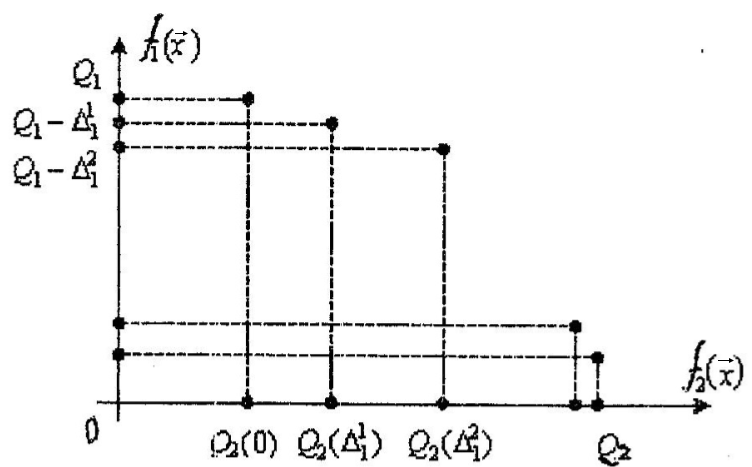
\includegraphics[width=0.6\textwidth]{figures/example_q2}
  \caption{Графік функцій обмежень}
  \label{fig:example_q2}
\end{figure}

На рисунку показано, що спочатку навіть невеликі величини поступок за першим критерієм можуть дозволити одержати істотний виграш за другим критерієм.
Подальше істотне збільшення поступки за першим критерієм може приводити до більш повільного зростання виграшу за другим критерієм.
На підставі аналізу отриманих даних і вирішують питання про призначення величини поступки $\Delta_1$, а потім знаходять $Q_2(\Delta_1)$.

Далі розглядають пари критеріїв $f_2(\vec{x})$ і $f_3(\vec{x})$. 
Знову призначають <<пробні>> величини поступок $\Delta_2^1$, $\Delta_2^2$, $\dots$ і, розв'язуючи третью задачу~\eqref{eq:qm}, відшукують найкращі значення третього критерію $Q_3(\Delta_2^1)$, $Q_3(\Delta_2^2)$, \dots. 
Отримані дані аналізують, призначають $\Delta_2$, переходять до наступної пари критеріїв $f_3(\vec{x})$, $f_4(\vec{x})$ і так далі.

Нарешті, у результаті аналізу взаємного впливу критеріїв $f_{M-1}(\vec{x})$ і $f_{M}(\vec{x})$ вибирають величину останньої поступки $\Delta_{M-1}$ і відшукують оптимальні стратегії, розв'язуючи задачу~\eqref{eq:qm}. 
Зазвичай обмежуються знаходженням однієї такої стратегії.

Таким чином, хоча формально при використанні методу послідовних поступок досить розв'язати лише $M$ задач вигляду~\eqref{eq:q1},~\eqref{eq:q2}, \dots ,~\eqref{eq:qm}, однак для призначення величин поступок з метою з'ясування взаємозв'язку окремих критеріїв фактично доводиться розв'язувати істотно більше число подібних задач.

\subsection{Математична постановка вихідної багатокритеріальної згідно до виданого завдання}
Для виданого завдання задачі~\eqref{eq:q1},~\eqref{eq:q2} та~\eqref{eq:qm} приймуть вигляд:
\begin{enumerate}[label=\arabic*)]
	\item знайти: 
	\[
		Q_1 = \max_{\vec{x} \in A} x_1;
	\]
	\item знайти:
	\[
		Q_2 = \max_{D_M} x_2,
	\]
	\begin{gather*}
		D_2= \begin{cases} 
			\vec{x} \in A, \\
			f_i(\vec{x}) \geq Q_i - \Delta_i, & i \in I_1;  
		\end{cases}
	\end{gather*}
	\dotfill
	\item[$M$)] знайти: 
	\[
		Q_M = \max_{D_M} x_3
	\]
	\[
		D_M = \begin{cases}
			\vec{x} \in A, \\
			f_i(\vec{x}) \geq Q_i - \Delta_i, & i \in I_1.
		\end{cases}
	\]
\end{enumerate}

Результати розрахунків були занесені до таблиці~\ref{tab:result}.
Графічна інтерпретація розрахунків представлена на рисунках~\ref{fig:results1} та~\ref{fig:results2}.

\clearpage
\begin{table}[H]        
    \caption{Результати розрахунків}
	\label{tab:result}
    \small
\begin{tabular}{c|cccccc}
	$i$ & 1 & 2 & 3 & 4 & 5 & 6 \\
	\hline
	$\Delta_1^i$ & 0.5 & 1 & 1.5 & 2 & 2.5 & 3 \\
	$f_1(\vec{x})$ & 3.5&	3	&2.5	&2	&1.5	&1 \\
	$f_2(\vec{x})$ & 0.5&	1	&1.5&	2	&2.125&	2.25 \\
	\hline
	\multicolumn{7}{c}{$f_1=3.5$, $\Delta_1^1=0.5$} \\
	\hline
	$\Delta_2^i$ & 0.01&	0.02&	0.04&	0.08&	0.16&	0.32 \\
	$f_2(\vec{x})$ & 0.49&	0.48&	0.46&	0.42&	0.34&	0.18 \\
	$f_3(\vec{x})$ & 0.01&	0.02&	0.04&	0.08&	0.16&	0.32 \\
	\hline
	\multicolumn{7}{c}{$f_1=3$, $\Delta_1^2=1.0$} \\
	\hline
	$\Delta_2^i$ & 0.1&	0.2&	0.3&	0.4&	0.5&	0.6 \\
	$f_2(\vec{x})$ & 0.9&	0.8&	0.7&	0.6&	0.5&	0.4 \\
	$f_3(\vec{x})$ & 0.1&	0.2&	0.3&	0.4&	0.5&	0.6 \\
	\hline
	\multicolumn{7}{c}{$f_1=2.5$, $\Delta_1^3=1.5$} \\
	\hline
	$\Delta_2^i$ & 0.15&	0.3&	0.45&	0.6&	0.75&	0.9 \\
	$f_2(\vec{x})$ & 1.35&	1.2&	1.05&	0.9&	0.75&	0.6 \\
	$f_3(\vec{x})$ & 0.15&	0.3&	0.45&	0.6&	0.75&	0.9 \\
	\hline
	\multicolumn{7}{c}{$f_1=2.0$, $\Delta_1^4=2.0$} \\
	\hline
	$\Delta_2^i$ & 0.2&	0.4&	0.6&	0.8&	1.0&	1.2 \\
	$f_2(\vec{x})$ & 1.8&	1.6&	1.4&	1.2&	1.0&	0.8 \\
	$f_3(\vec{x})$ & 0.2&	0.4&	0.6&	0.8&	1.0&	1.2 \\
	\hline
	\multicolumn{7}{c}{$f_1=1.5$, $\Delta_1^5=2.125$} \\
	\hline
	$\Delta_2^i$ & 0.25&	0.5&	0.75&	1.0&	1.25&	1.5 \\
	$f_2(\vec{x})$ & 1.875&	1.625&	1.375&	1.125&	0.875&	0.625 \\
	$f_3(\vec{x})$ & 0.625&	0.875&	1.125&	1.375&	1.625&	1.875 \\
	\hline
	\multicolumn{7}{c}{$f_1=1$, $\Delta_1^6=2.25$} \\
	\hline
	$\Delta_2^i$ & 0.3&	0.6&	0.9&	1.2&	1.5&	1.8 \\
	$f_2(\vec{x})$ & 1.95&	1.65&	1.35&	1.05&	0.75&	0.45 \\
	$f_3(\vec{x})$ & 0.55&	0.85&	1.15&	1.45&	1.75&	2.05 \\
\end{tabular}
\end{table}

\begin{landscape}
\begin{figure*}[t!]
    \centering
    \begin{subfigure}[t]{0.33\linewidth}

\begin{tikzpicture}
\begin{axis}[
    xlabel={$f_1(\vec{x})$},
    ylabel={$f_2(\vec{x})$},
]
\node[above] at (axis cs:3.5, 0.5) {\footnotesize $\Delta_1^1 = 0.5$};
\node[above] at (axis cs:3.0, 1.0) {\footnotesize $\Delta_1^2 = 1.0$};
\node[above] at (axis cs:2.5, 1.5) {\footnotesize $\Delta_1^3 = 1.5$};
\node[above] at (axis cs:2.0, 2.0) {\footnotesize $\Delta_1^4 = 2.0$};
\node[above] at (axis cs:1.5, 2.125) {\footnotesize $\Delta_1^5 = 2.5$};
\node[above] at (axis cs:1.0, 2.25) {\footnotesize $\Delta_1^6 = 3.0$};
\addplot[
    color=red,
    mark=*,
    ]
    coordinates {
    (3.5, 0.5) (3.0, 1.0) (2.5, 1.5) (2.0, 2.0) (1.5, 2.125) (1.0, 2.25)  
    };

\end{axis}
\end{tikzpicture}

    \end{subfigure}
    ~
    \begin{subfigure}[t]{0.33\linewidth}

\begin{tikzpicture}
\begin{axis}[
    xlabel={$f_2(\vec{x})$},
    ylabel={$f_3(\vec{x})$},
]
\node[above] at (axis cs:0.18, 0.32) {\footnotesize $\Delta_2^6 = 0.32$};
\node[above] at (axis cs:0.34, 0.16) {\footnotesize $\Delta_2^5 = 0.16$};
\node[above] at (axis cs:0.42, 0.08) {\footnotesize $\Delta_2^4 = 0.08$};
\node[above] at (axis cs:0.46, 0.04) {\footnotesize $\Delta_2^3 = 0.04$};
\node[above] at (axis cs:0.48, 0.02) {\footnotesize $\Delta_2^2 = 0.02$};
\node[above] at (axis cs:0.49, 0.01) {\footnotesize $\Delta_2^1 = 0.01$};
\addplot[
    color=blue,
    mark=*,
    ]
    coordinates {
    (0.18, 0.32) (0.34, 0.16) (0.42, 0.08) (0.46, 0.04) (0.48, 0.02) (0.49, 0.01)  
    };
    \legend{$f_1 = 3.5$; $\Delta_1^1=0.5$}

\end{axis}
\end{tikzpicture}

    \end{subfigure}
    ~
    \begin{subfigure}[t]{0.33\linewidth}
 
\begin{tikzpicture}
\begin{axis}[
    xlabel={$f_2(\vec{x})$},
    ylabel={$f_3(\vec{x})$},
]
\node[above] at (axis cs:0.4, 0.6) {\footnotesize $\Delta_2^6 = 0.6$};
\node[above] at (axis cs:0.5, 0.5) {\footnotesize $\Delta_2^5 = 0.5$};
\node[above] at (axis cs:0.6, 0.4) {\footnotesize $\Delta_2^4 = 0.4$};
\node[above] at (axis cs:0.7, 0.3) {\footnotesize $\Delta_2^3 = 0.3$};
\node[above] at (axis cs:0.8, 0.2) {\footnotesize $\Delta_2^2 = 0.2$};
\node[above] at (axis cs:0.9, 0.1) {\footnotesize $\Delta_2^1 = 0.1$};
\addplot[
    color=blue,
    mark=*,
    ]
    coordinates {
    (0.9, 0.1) (0.8, 0.2) (0.7, 0.3) (0.6, 0.4) (0.5, 0.5) (0.4, 0.6)
    };
    \legend{$f_1 = 3$; $\Delta_1^2=1.0$}

\end{axis}
\end{tikzpicture}

    \end{subfigure}
    ~
    \begin{subfigure}[t]{0.33\linewidth}
 
\begin{tikzpicture}
\begin{axis}[
    xlabel={$f_2(\vec{x})$},
    ylabel={$f_3(\vec{x})$},
]
\node[above] at (axis cs:1.35, 0.15) {\footnotesize $\Delta_2^1 = 0.15$};
\node[above] at (axis cs:1.2, 0.3) {\footnotesize $\Delta_2^2 = 0.3$};
\node[above] at (axis cs:1.05, 0.45) {\footnotesize $\Delta_2^3 = 0.45$};
\node[above] at (axis cs:0.9, 0.6) {\footnotesize $\Delta_2^4 = 0.6$};
\node[above] at (axis cs:0.75, 0.75) {\footnotesize $\Delta_2^5 = 0.75$};
\node[above] at (axis cs:0.6, 0.9) {\footnotesize $\Delta_2^6 = 0.9$};
\addplot[
    color=blue,
    mark=*,
    ]
    coordinates {
    (1.35, 0.15) (1.2, 0.3) (1.05, 0.45) (0.9, 0.6) (0.75, 0.75) (0.6, 0.9)
    };
    \legend{$f_1 = 2.5$; $\Delta_1^3=1.5$}

\end{axis}
\end{tikzpicture}

    \end{subfigure}
    \caption{Результати розрахунків}
    \label{fig:results1}
\end{figure*}

\begin{figure*}[t!]
    \centering
    \begin{subfigure}[t]{0.33\linewidth}
 
\begin{tikzpicture}
\begin{axis}[
    xlabel={$f_2(\vec{x})$},
    ylabel={$f_3(\vec{x})$},
]
\node[above] at (axis cs:1.8, 0.2) {\footnotesize $\Delta_2^1 = 0.2$};
\node[above] at (axis cs:1.6, 0.4) {\footnotesize $\Delta_2^2 = 0.4$};
\node[above] at (axis cs:1.4, 0.6) {\footnotesize $\Delta_2^3 = 0.6$};
\node[above] at (axis cs:1.2, 0.8) {\footnotesize $\Delta_2^4 = 0.8$};
\node[above] at (axis cs:1, 1) {\footnotesize $\Delta_2^5 = 1.0$};
\node[above] at (axis cs:0.8, 1.2) {\footnotesize $\Delta_2^6 = 1.2$};
\addplot[
    color=blue,
    mark=*,
    ]
    coordinates {
    (1.8, 0.2) (1.6, 0.4) (1.4, 0.6) (1.2, 0.8) (1, 1) (0.8, 1.2)
    };
    \legend{$f_1 = 2$; $\Delta_1^4=2.0$}

\end{axis}
\end{tikzpicture}

    \end{subfigure}
    ~
    \begin{subfigure}[t]{0.33\linewidth}
 
\begin{tikzpicture}
\begin{axis}[
    xlabel={$f_2(\vec{x})$},
    ylabel={$f_3(\vec{x})$},
]
\node[above] at (axis cs:1.875, 0.625) {\footnotesize $\Delta_2^1 = 0.25$};
\node[above] at (axis cs:1.625, 0.875) {\footnotesize $\Delta_2^2 = 0.5$};
\node[above] at (axis cs:1.375, 1.125) {\footnotesize $\Delta_2^3 = 0.75$};
\node[above] at (axis cs:1.125, 1.375) {\footnotesize $\Delta_2^4 = 1.0$};
\node[above] at (axis cs:0.875, 1.625) {\footnotesize $\Delta_2^5 = 1.25$};
\node[above] at (axis cs:0.625, 1.875) {\footnotesize $\Delta_2^6 = 1.5$};
\addplot[
    color=blue,
    mark=*,
    ]
    coordinates {
    (1.875, 0.625) (1.625, 0.875) (1.375, 1.125) (1.125, 1.375) (0.875, 1.625) (0.625, 1.875)
    };
    \legend{$f_1 = 1.5$; $\Delta_1^5=2.5$}

\end{axis}
\end{tikzpicture}

    \end{subfigure}
    ~
    \begin{subfigure}[t]{0.33\linewidth}
 
\begin{tikzpicture}
\begin{axis}[
    xlabel={$f_2(\vec{x})$},
    ylabel={$f_3(\vec{x})$},
]
\node[above] at (axis cs:1.95, 0.55) {\footnotesize $\Delta_2^1 = 0.3$};
\node[above] at (axis cs:1.65, 0.85) {\footnotesize $\Delta_2^2 = 0.6$};
\node[above] at (axis cs:1.35, 1.15) {\footnotesize $\Delta_2^3 = 0.9$};
\node[above] at (axis cs:1.05, 1.45) {\footnotesize $\Delta_2^4 = 1.2$};
\node[above] at (axis cs:0.75, 1.75) {\footnotesize $\Delta_2^5 = 1.5$};
\node[above] at (axis cs:0.45, 2.05) {\footnotesize $\Delta_2^6 = 1.8$};
\addplot[
    color=blue,
    mark=*,
    ]
    coordinates {
    (1.95, 0.55) (1.65, 0.85) (1.35, 1.15) (1.05, 1.45) (0.75, 1.75) (0.45, 2.05)
    };
    \legend{$f_1 = 1$; $\Delta_1^6=3.0$}

\end{axis}
\end{tikzpicture}

    \end{subfigure}
    \caption{Результати розрахунків}
    \label{fig:results2}
\end{figure*}

\end{landscape}

\subsection{Висновки}
В ході виконання лабораторної роботи було вивчено загальні положення методу поступок. 
Вихідні критерії були впорядковані за важливістю, після чого виконувався підбір можливих поступок для кожного критерію, крім останнього, та оцінювався їх вплив на значення менш важливих критеріїв.

Було встановлено, що невеликі поступки дозволяють зберегти більш сприятливі значення головних критеріїв, в той час як введення великих поступок дозволяє досягти більш кращих значень незначних критеріїв.

\end{document}